\documentclass[letterpaper,twoside,12pt]{article}
\usepackage{graphicx}
\usepackage[margin=0.8in]{geometry}


\title{ER2201 Session Delay Closures}
%\author[1]{L. Benkevitch}

\begin{document}

\maketitle

Figs.~\ref{mbd} and~\ref{sbd} show closure delay distributions over 5.5 hours and histograms of absolute magnitudes for the multi-band and single-band delays and their residuals.

The closure delay calculations of the total multi-band and single-band delays fail for EVY, EMY, ESY, ETY, MSY, MTY, MVY, SVY, TVY triangles. However, the delay closures for triangles EMV, ESV, ETV, EMS, EMT, MSV, MTV demonstrate good behavior. Figs.~\ref{tot_mbd} and~\ref{tot_sbd} show the total mbd and sbd closures for for $|\tau| < 500 ps$ and $|\tau| > 500 ps$ separately. 

The legend for colored dots in the closure delay distributions is shown in Fig.~\ref{col_legend}.


\begin{figure}[h!]
  %\begin{center}
  \centering
  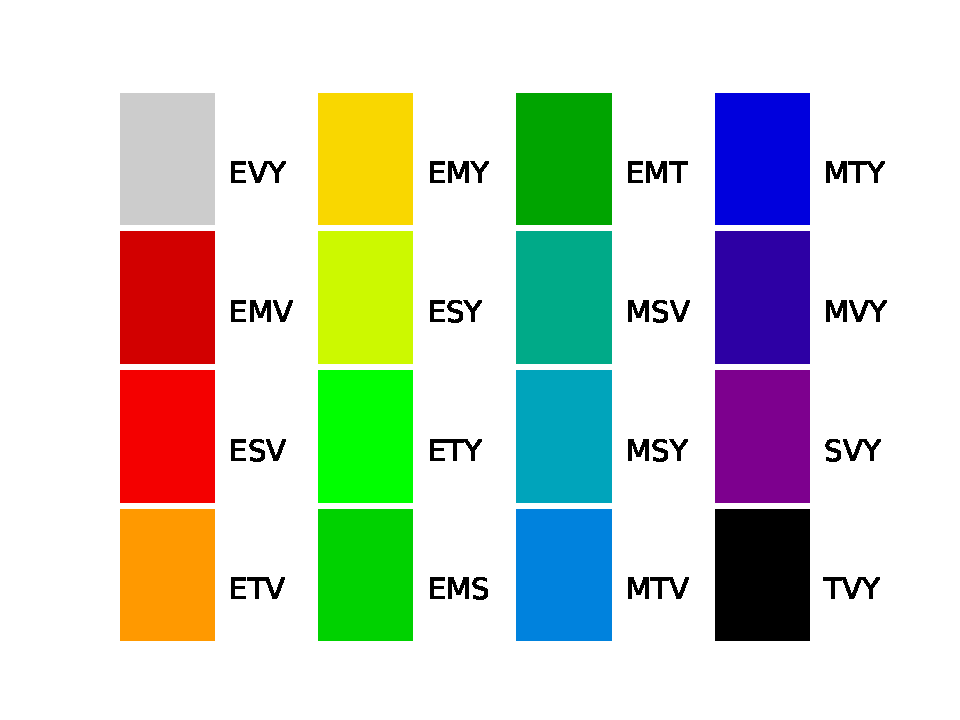
\includegraphics[width=20pc]{Triangle_color_legend.pdf}
  \caption{\small Color legend for the closure triangles.}
  \label{col_legend}
  %\end{center}
\end{figure}


\begin{figure}[h!]
  %\begin{center}
  \centering
  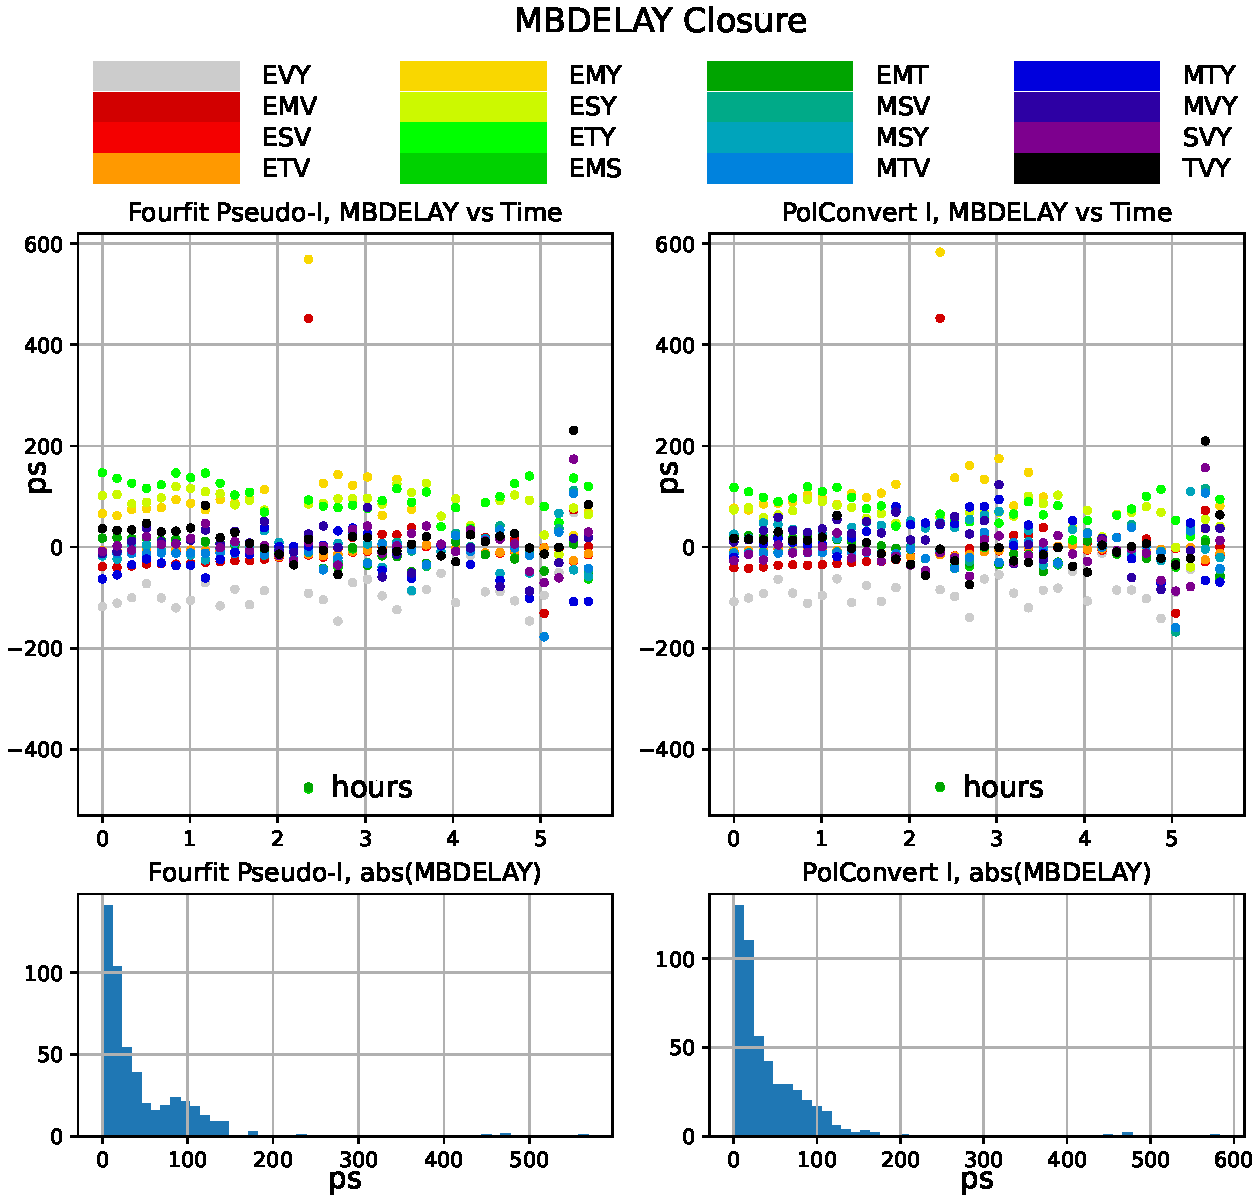
\includegraphics[width=35pc]{MBDELAY_Closure_Delay.pdf}
  \caption{\small MBDELAY closure delay distributions over 5.5 hours and histograms of their absolute magnitudes.}
  \label{mbd}
  %\end{center}
\end{figure}


\begin{figure}[ht!]
  \begin{center}
  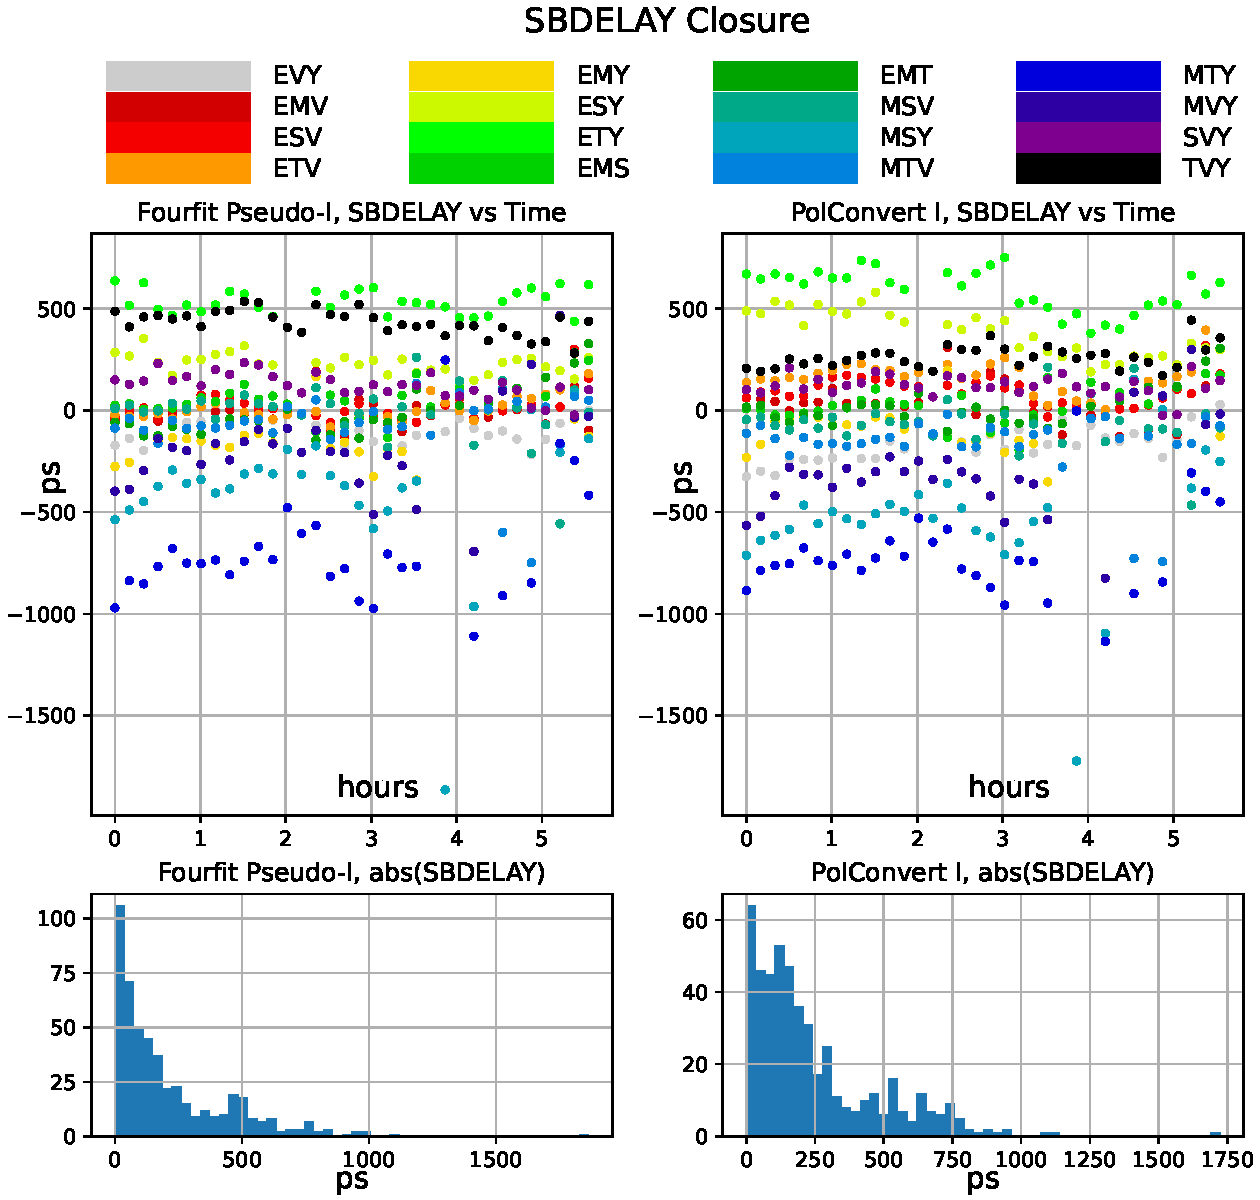
\includegraphics[width=35pc]{SBDELAY_Closure_Delay.pdf}
  \caption{\small SBDELAY closure delay distributions over 5.5 hours and histograms of their absolute magnitudes.}
  \label{sbd}
  \end{center}
\end{figure}


\begin{figure}[ht!]
  \begin{center}
  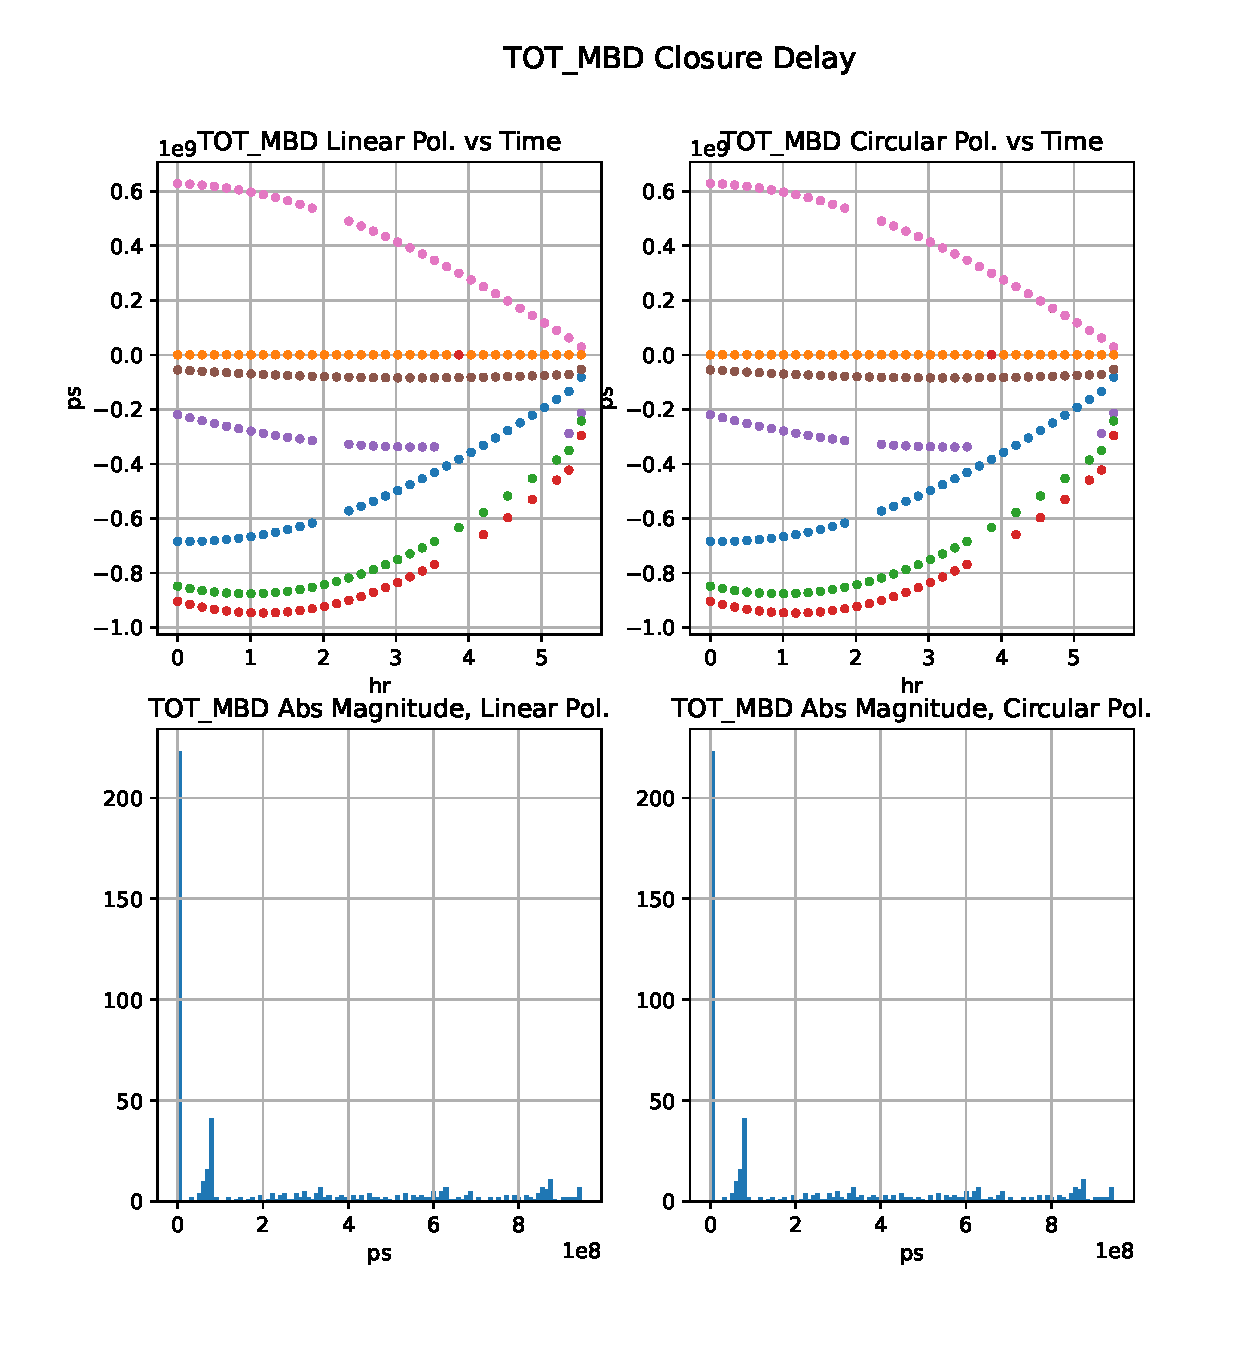
\includegraphics[width=35pc]{TOT_MBD_Closure_Delay.pdf}
  \caption{\small Total MBDELAY closure delay distributions over 5.5 hours and histograms of their absolute magnitudes.}
  \label{tot_mbd}
  \end{center}
\end{figure}


\begin{figure}[ht!]
  \begin{center}
  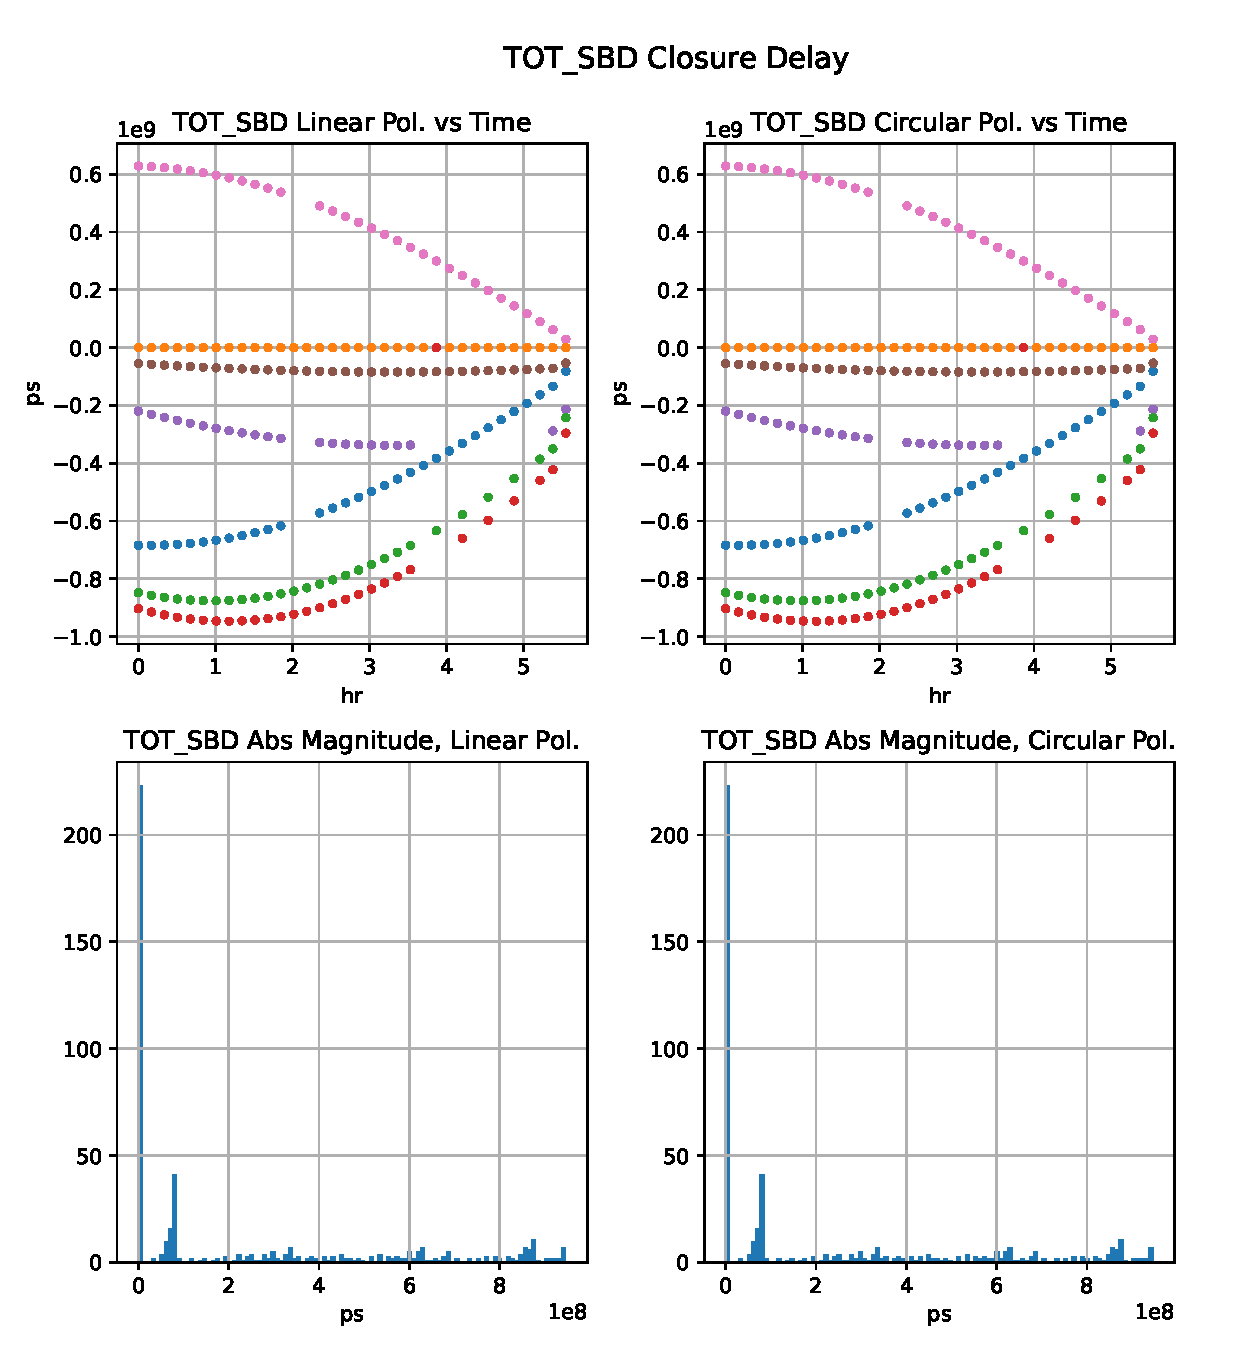
\includegraphics[width=35pc]{TOT_SBD_Closure_Delay.pdf}
  \caption{\small Total SBDELAY closure delay distributions over 5.5 hours and histograms of their absolute magnitudes.}
  \label{tot_sbd}
  \end{center}
\end{figure}




\end{document}








